\chapter{Evaluation}
\label{chap:evaluation}
% "Moreover, under large record size (e.g., 1KB and above), B+ tree tend to have smaller write amplification than LSM-tree." - from "Closing the B+-Tree vs. LSM-Tree Write Amplification Gap on Modern Storage Hardware with Built-in Transparent Compression", Qiao et al., FAST 2022
% Good evaluation paper: https://dl.acm.org/doi/pdf/10.1145/3183713.3196895
% To adhere to the DAM model, can't we assume that all inner nodes are cached in memory, but leafs are not? see "A Comparison of Fractal Trees to Log-Structured Merge (LSM) Trees"

% Question 0: How much write amplification do we have in a traditional B-tree. How much in our approach? Show the bytes inserted by the user, the bytes written to the tree, the bytes written to storage.
% Question 1: Does the approach reduce write amplification compared to a traditional B-Tree?
% Question 2: How does the approach affect read and write performance compared to a traditional B-Tree and LSM-Tree?
% Question 3: How does the approach affect latency/throughput?
% Question 4: How does the approach affect space utilization?
% Question 5: How does the approach affect memory usage and CPU utilization?
% Question 6: How does the approach scale with different types of workloads (read-heavy, write-heavy, mixed)?
% Question 7: How does the approach perform with different types of page sizes and delta sizes?

% Observations:
% We write a lot in the Delta Tree, to delete entries. Less fanout if we dont compactify often enough.

\section{Experimental Setup}
% Hardware specs
% Dataset, distribution
% Workloads (insert-heavy, read-heavy, mixed)
% Baselines (B-Tree, LSM-Tree)
% Metrics (write amplification, throughput (ops/s), latency, space utilization, memory usage, CPU utilization)

\section{Results and Analysis}
\subsection*{Write Amplification}

\begin{figure}[htbp]
  \centering
  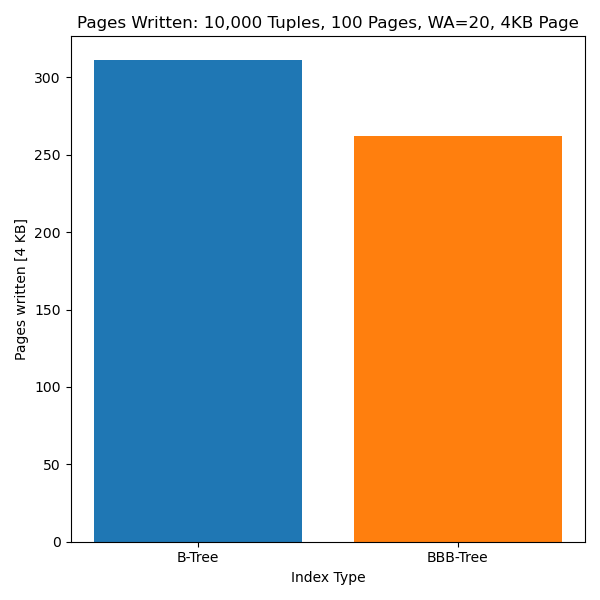
\includegraphics[width=0.6\textwidth]{figures/evaluation/10K_tuples_20_wa.png}
  \caption{Comparison of B-Tree and BBBTree performance for 10,000 insertions, building the index from scratch. We observe 15\% reduction in write amplification with our approach.}
  \label{fig:btree-vs-bbbtree-10000}
\end{figure}


\begin{figure}[htbp]
  \centering
  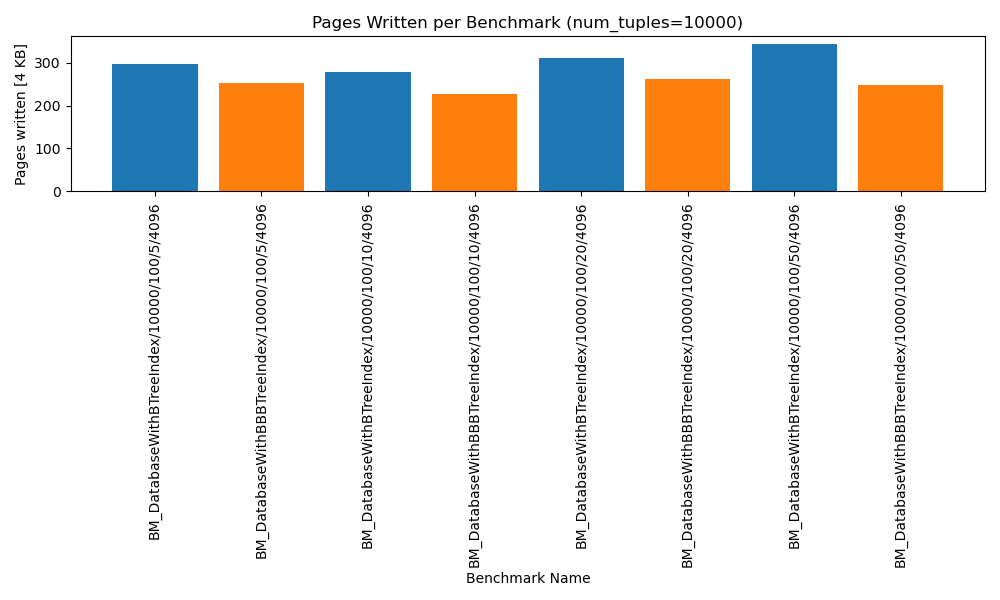
\includegraphics[width=0.8\textwidth]{figures/evaluation/10K_tuples_all_wa.png}
  \caption{Comparison of B-Tree and BBBTree performance for 10,000 insertions, building the index from scratch. We observe reduction in write amplification across different write amplification thresholds.}
  \label{fig:btree-vs-bbbtree-10000-all-wa}
\end{figure}

\begin{figure}[htbp]
  \centering
  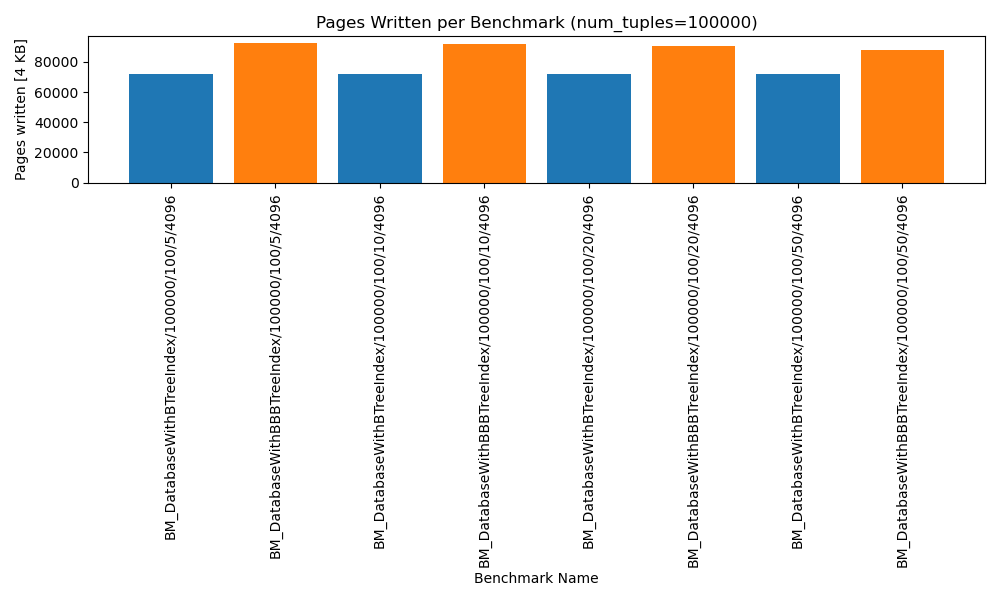
\includegraphics[width=0.8\textwidth]{figures/evaluation/100K_tuples_all_wa.png}
  \caption{Comparison of B-Tree and BBBTree performance for 100,000 insertions, building the index from scratch. We observe increase in write amplification across different write amplification thresholds.}
  \label{fig:btree-vs-bbbtree-100000-all-wa}
\end{figure}

% Write Amplification vs. Data size
% Write Amplification vs. Workload type (read-heavy, write-heavy, mixed)
% Number of writes to storage vs. workload type
% Average IO operations per update (baseline vs. our approach)

\subsection*{Latency and Throughput}
% Latency vs. Workload type
% Throughput vs. Workload type
% Latency vs. Data size
% Throughput vs. Data size

\subsection*{Space Utilization and Memory Overhead}
% Space Utilization vs. Data size (probably need more pages for fewer entries because slot size increases with delta tracking)
% 

\subsection*{Sensitivity Analysis}
% WA vs Key Size
% WA vs Page Size
% WA vs Buffer Size
% WA vs Delta Size

\section{Discussion}
% “Our approach reduces write amplification by 40–60% while maintaining within 5% of baseline read latency.”